\documentclass[]{article}
\usepackage{lmodern}
\usepackage{amssymb,amsmath}
\usepackage{ifxetex,ifluatex}
\usepackage{fixltx2e} % provides \textsubscript
\ifnum 0\ifxetex 1\fi\ifluatex 1\fi=0 % if pdftex
  \usepackage[T1]{fontenc}
  \usepackage[utf8]{inputenc}
\else % if luatex or xelatex
  \ifxetex
    \usepackage{mathspec}
  \else
    \usepackage{fontspec}
  \fi
  \defaultfontfeatures{Ligatures=TeX,Scale=MatchLowercase}
\fi
% use upquote if available, for straight quotes in verbatim environments
\IfFileExists{upquote.sty}{\usepackage{upquote}}{}
% use microtype if available
\IfFileExists{microtype.sty}{%
\usepackage{microtype}
\UseMicrotypeSet[protrusion]{basicmath} % disable protrusion for tt fonts
}{}
\usepackage[margin=1in]{geometry}
\usepackage{hyperref}
\hypersetup{unicode=true,
            pdftitle={R Notebook},
            pdfauthor={Alex Verkerk},
            pdfborder={0 0 0},
            breaklinks=true}
\urlstyle{same}  % don't use monospace font for urls
\usepackage{color}
\usepackage{fancyvrb}
\newcommand{\VerbBar}{|}
\newcommand{\VERB}{\Verb[commandchars=\\\{\}]}
\DefineVerbatimEnvironment{Highlighting}{Verbatim}{commandchars=\\\{\}}
% Add ',fontsize=\small' for more characters per line
\usepackage{framed}
\definecolor{shadecolor}{RGB}{248,248,248}
\newenvironment{Shaded}{\begin{snugshade}}{\end{snugshade}}
\newcommand{\AlertTok}[1]{\textcolor[rgb]{0.94,0.16,0.16}{#1}}
\newcommand{\AnnotationTok}[1]{\textcolor[rgb]{0.56,0.35,0.01}{\textbf{\textit{#1}}}}
\newcommand{\AttributeTok}[1]{\textcolor[rgb]{0.77,0.63,0.00}{#1}}
\newcommand{\BaseNTok}[1]{\textcolor[rgb]{0.00,0.00,0.81}{#1}}
\newcommand{\BuiltInTok}[1]{#1}
\newcommand{\CharTok}[1]{\textcolor[rgb]{0.31,0.60,0.02}{#1}}
\newcommand{\CommentTok}[1]{\textcolor[rgb]{0.56,0.35,0.01}{\textit{#1}}}
\newcommand{\CommentVarTok}[1]{\textcolor[rgb]{0.56,0.35,0.01}{\textbf{\textit{#1}}}}
\newcommand{\ConstantTok}[1]{\textcolor[rgb]{0.00,0.00,0.00}{#1}}
\newcommand{\ControlFlowTok}[1]{\textcolor[rgb]{0.13,0.29,0.53}{\textbf{#1}}}
\newcommand{\DataTypeTok}[1]{\textcolor[rgb]{0.13,0.29,0.53}{#1}}
\newcommand{\DecValTok}[1]{\textcolor[rgb]{0.00,0.00,0.81}{#1}}
\newcommand{\DocumentationTok}[1]{\textcolor[rgb]{0.56,0.35,0.01}{\textbf{\textit{#1}}}}
\newcommand{\ErrorTok}[1]{\textcolor[rgb]{0.64,0.00,0.00}{\textbf{#1}}}
\newcommand{\ExtensionTok}[1]{#1}
\newcommand{\FloatTok}[1]{\textcolor[rgb]{0.00,0.00,0.81}{#1}}
\newcommand{\FunctionTok}[1]{\textcolor[rgb]{0.00,0.00,0.00}{#1}}
\newcommand{\ImportTok}[1]{#1}
\newcommand{\InformationTok}[1]{\textcolor[rgb]{0.56,0.35,0.01}{\textbf{\textit{#1}}}}
\newcommand{\KeywordTok}[1]{\textcolor[rgb]{0.13,0.29,0.53}{\textbf{#1}}}
\newcommand{\NormalTok}[1]{#1}
\newcommand{\OperatorTok}[1]{\textcolor[rgb]{0.81,0.36,0.00}{\textbf{#1}}}
\newcommand{\OtherTok}[1]{\textcolor[rgb]{0.56,0.35,0.01}{#1}}
\newcommand{\PreprocessorTok}[1]{\textcolor[rgb]{0.56,0.35,0.01}{\textit{#1}}}
\newcommand{\RegionMarkerTok}[1]{#1}
\newcommand{\SpecialCharTok}[1]{\textcolor[rgb]{0.00,0.00,0.00}{#1}}
\newcommand{\SpecialStringTok}[1]{\textcolor[rgb]{0.31,0.60,0.02}{#1}}
\newcommand{\StringTok}[1]{\textcolor[rgb]{0.31,0.60,0.02}{#1}}
\newcommand{\VariableTok}[1]{\textcolor[rgb]{0.00,0.00,0.00}{#1}}
\newcommand{\VerbatimStringTok}[1]{\textcolor[rgb]{0.31,0.60,0.02}{#1}}
\newcommand{\WarningTok}[1]{\textcolor[rgb]{0.56,0.35,0.01}{\textbf{\textit{#1}}}}
\usepackage{graphicx,grffile}
\makeatletter
\def\maxwidth{\ifdim\Gin@nat@width>\linewidth\linewidth\else\Gin@nat@width\fi}
\def\maxheight{\ifdim\Gin@nat@height>\textheight\textheight\else\Gin@nat@height\fi}
\makeatother
% Scale images if necessary, so that they will not overflow the page
% margins by default, and it is still possible to overwrite the defaults
% using explicit options in \includegraphics[width, height, ...]{}
\setkeys{Gin}{width=\maxwidth,height=\maxheight,keepaspectratio}
\IfFileExists{parskip.sty}{%
\usepackage{parskip}
}{% else
\setlength{\parindent}{0pt}
\setlength{\parskip}{6pt plus 2pt minus 1pt}
}
\setlength{\emergencystretch}{3em}  % prevent overfull lines
\providecommand{\tightlist}{%
  \setlength{\itemsep}{0pt}\setlength{\parskip}{0pt}}
\setcounter{secnumdepth}{0}
% Redefines (sub)paragraphs to behave more like sections
\ifx\paragraph\undefined\else
\let\oldparagraph\paragraph
\renewcommand{\paragraph}[1]{\oldparagraph{#1}\mbox{}}
\fi
\ifx\subparagraph\undefined\else
\let\oldsubparagraph\subparagraph
\renewcommand{\subparagraph}[1]{\oldsubparagraph{#1}\mbox{}}
\fi

%%% Use protect on footnotes to avoid problems with footnotes in titles
\let\rmarkdownfootnote\footnote%
\def\footnote{\protect\rmarkdownfootnote}

%%% Change title format to be more compact
\usepackage{titling}

% Create subtitle command for use in maketitle
\providecommand{\subtitle}[1]{
  \posttitle{
    \begin{center}\large#1\end{center}
    }
}

\setlength{\droptitle}{-2em}

  \title{R Notebook}
    \pretitle{\vspace{\droptitle}\centering\huge}
  \posttitle{\par}
    \author{Alex Verkerk}
    \preauthor{\centering\large\emph}
  \postauthor{\par}
      \predate{\centering\large\emph}
  \postdate{\par}
    \date{17/05/2019}


\begin{document}
\maketitle

This is an \href{http://rmarkdown.rstudio.com}{R Markdown} Notebook.
When you execute code within the notebook, the results appear beneath
the code.

Try executing this chunk by clicking the \emph{Run} button within the
chunk or by placing your cursor inside it and pressing
\emph{Ctrl+Shift+Enter}.

Add a new chunk by clicking the \emph{Insert Chunk} button on the
toolbar or by pressing \emph{Ctrl+Alt+I}.

When you save the notebook, an HTML file containing the code and output
will be saved alongside it (click the \emph{Preview} button or press
\emph{Ctrl+Shift+K} to preview the HTML file).

The preview shows you a rendered HTML copy of the contents of the
editor. Consequently, unlike \emph{Knit}, \emph{Preview} does not run
any R code chunks. Instead, the output of the chunk when it was last run
in the editor is displayed.

\begin{Shaded}
\begin{Highlighting}[]
\KeywordTok{library}\NormalTok{(s20x)}
\CommentTok{#laptop:/}
\CommentTok{#setwd("C:/Users/Alex/Documents/GitHub/Engsci211Assignment2")}
\CommentTok{#home computer:}
\KeywordTok{setwd}\NormalTok{(}\StringTok{"I:/GitHub/Engsci 211/Engsci211Assignment2"}\NormalTok{)}
\NormalTok{delays.df =}\StringTok{ }\KeywordTok{read.table}\NormalTok{(}\StringTok{"delays.txt"}\NormalTok{, }\DataTypeTok{header =} \OtherTok{TRUE}\NormalTok{)}
\KeywordTok{head}\NormalTok{(delays.df)}
\end{Highlighting}
\end{Shaded}

\begin{verbatim}
##    airline dep_delay
## 1 American       652
## 2 American         4
## 3 American       142
## 4 American       302
## 5 American         1
## 6 American        57
\end{verbatim}

\begin{Shaded}
\begin{Highlighting}[]
\KeywordTok{plot}\NormalTok{(dep_delay}\OperatorTok{~}\NormalTok{airline, }\DataTypeTok{data =}\NormalTok{ delays.df)}
\end{Highlighting}
\end{Shaded}

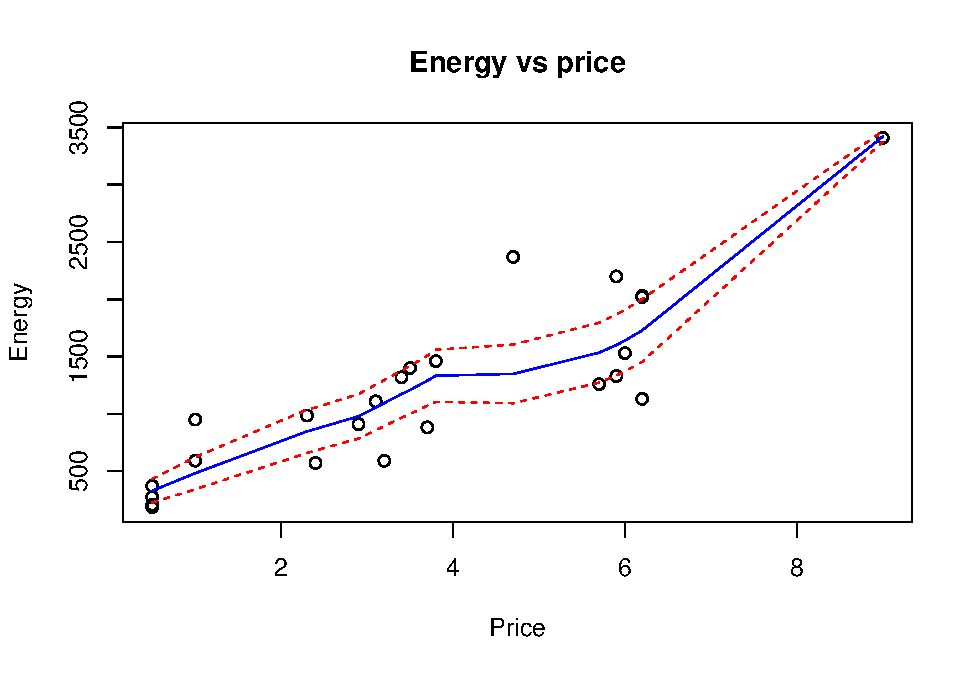
\includegraphics{Engsci211assignment2_task3_files/figure-latex/unnamed-chunk-2-1.pdf}

\begin{Shaded}
\begin{Highlighting}[]
\NormalTok{delays.fit =}\StringTok{ }\KeywordTok{lm}\NormalTok{(dep_delay}\OperatorTok{~}\NormalTok{airline, }\DataTypeTok{data =}\NormalTok{ delays.df)}
\KeywordTok{eovcheck}\NormalTok{(delays.fit)}
\end{Highlighting}
\end{Shaded}

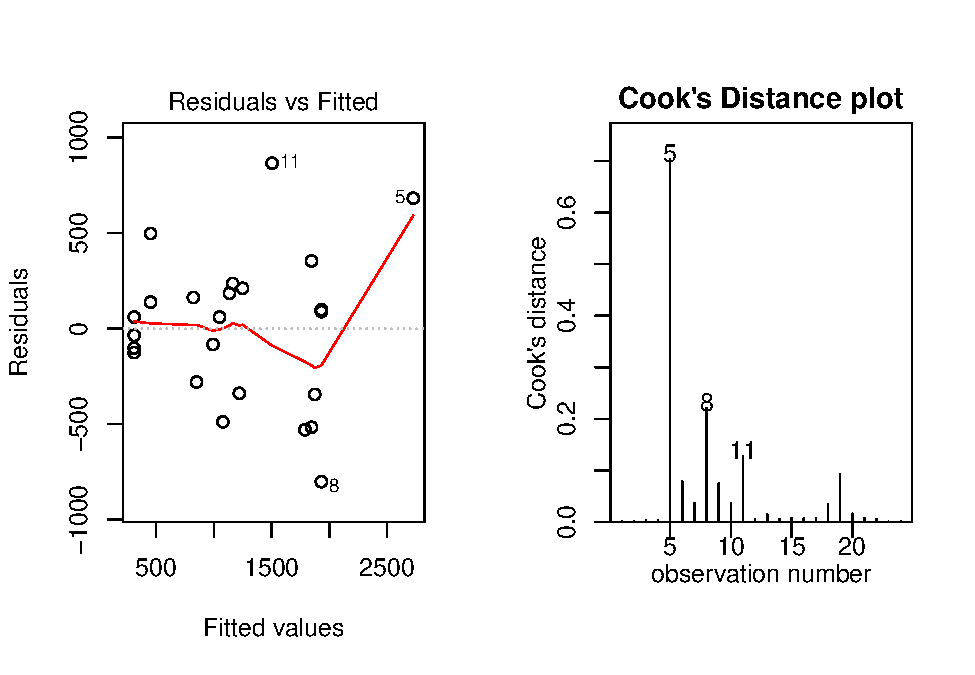
\includegraphics{Engsci211assignment2_task3_files/figure-latex/unnamed-chunk-3-1.pdf}

\begin{Shaded}
\begin{Highlighting}[]
\KeywordTok{normcheck}\NormalTok{(delays.fit)}
\end{Highlighting}
\end{Shaded}

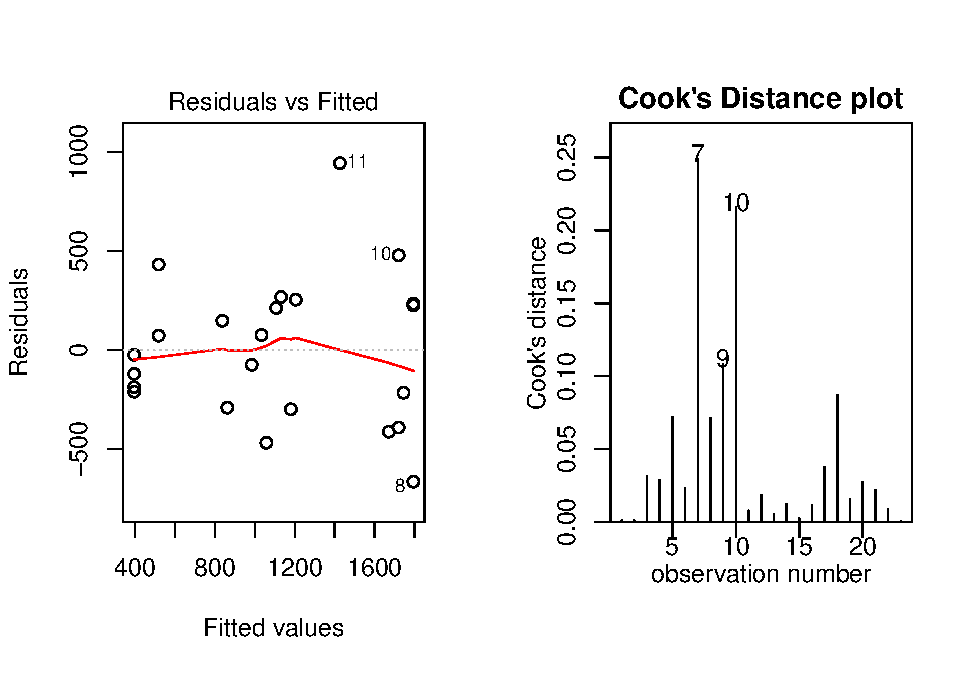
\includegraphics{Engsci211assignment2_task3_files/figure-latex/unnamed-chunk-4-1.pdf}

\begin{Shaded}
\begin{Highlighting}[]
\NormalTok{delays.fit2 =}\StringTok{ }\KeywordTok{lm}\NormalTok{(}\KeywordTok{log}\NormalTok{(dep_delay)}\OperatorTok{~}\NormalTok{airline,}\DataTypeTok{data=}\NormalTok{delays.df)}
\KeywordTok{eovcheck}\NormalTok{(delays.fit2)}
\end{Highlighting}
\end{Shaded}

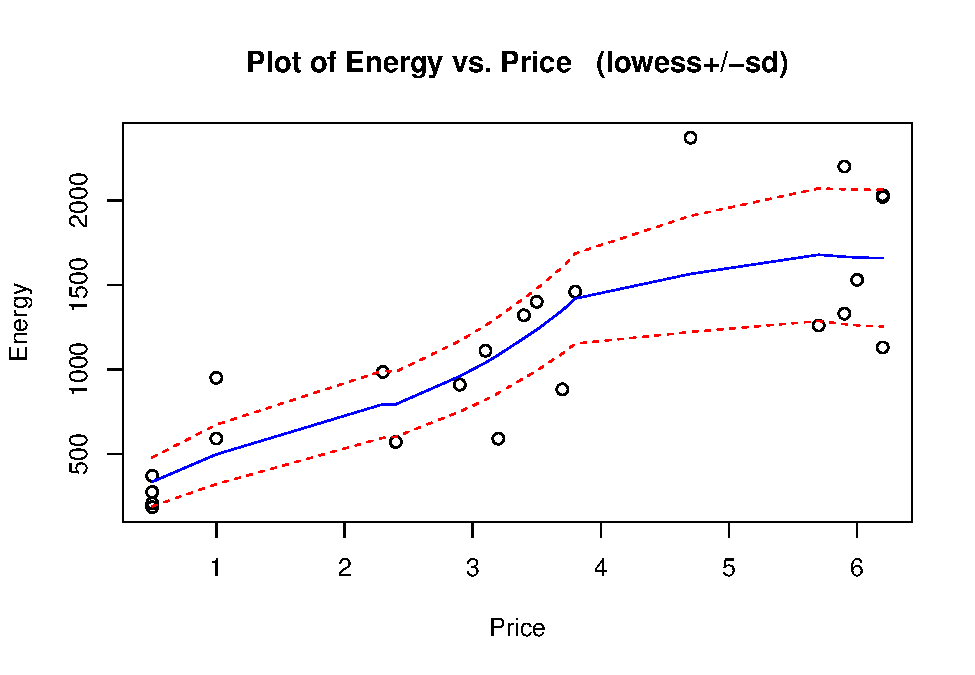
\includegraphics{Engsci211assignment2_task3_files/figure-latex/unnamed-chunk-5-1.pdf}

\begin{Shaded}
\begin{Highlighting}[]
\KeywordTok{normcheck}\NormalTok{(delays.fit2,}\DataTypeTok{shapiro.wilk =} \OtherTok{TRUE}\NormalTok{)}
\end{Highlighting}
\end{Shaded}

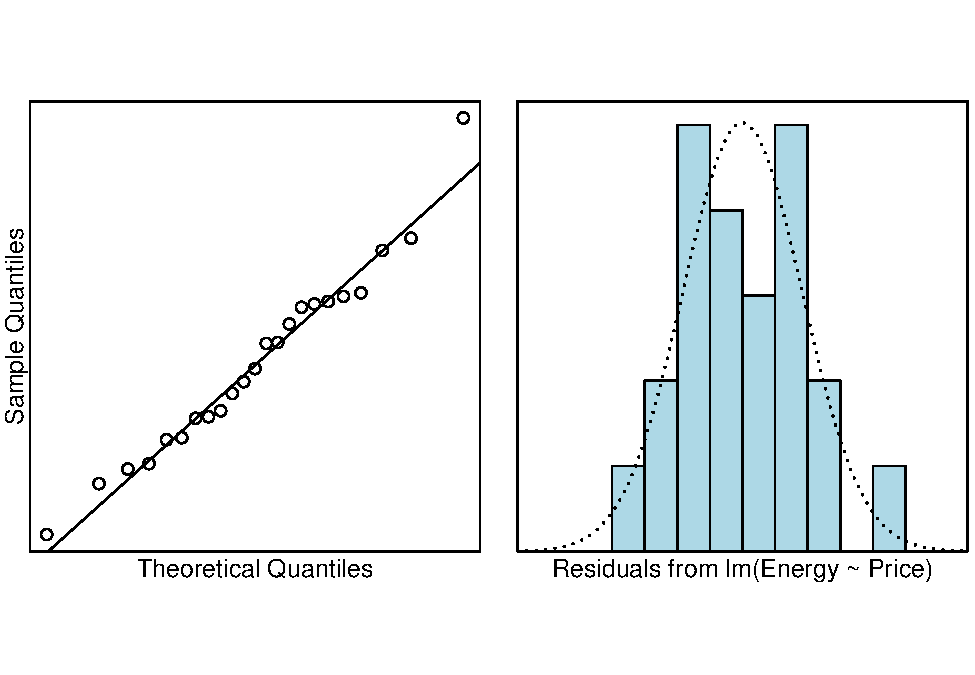
\includegraphics{Engsci211assignment2_task3_files/figure-latex/unnamed-chunk-6-1.pdf}

\begin{Shaded}
\begin{Highlighting}[]
\KeywordTok{boxplot}\NormalTok{(}\KeywordTok{log}\NormalTok{(dep_delay)}\OperatorTok{~}\NormalTok{airline, }\DataTypeTok{data =}\NormalTok{ delays.df)}
\end{Highlighting}
\end{Shaded}

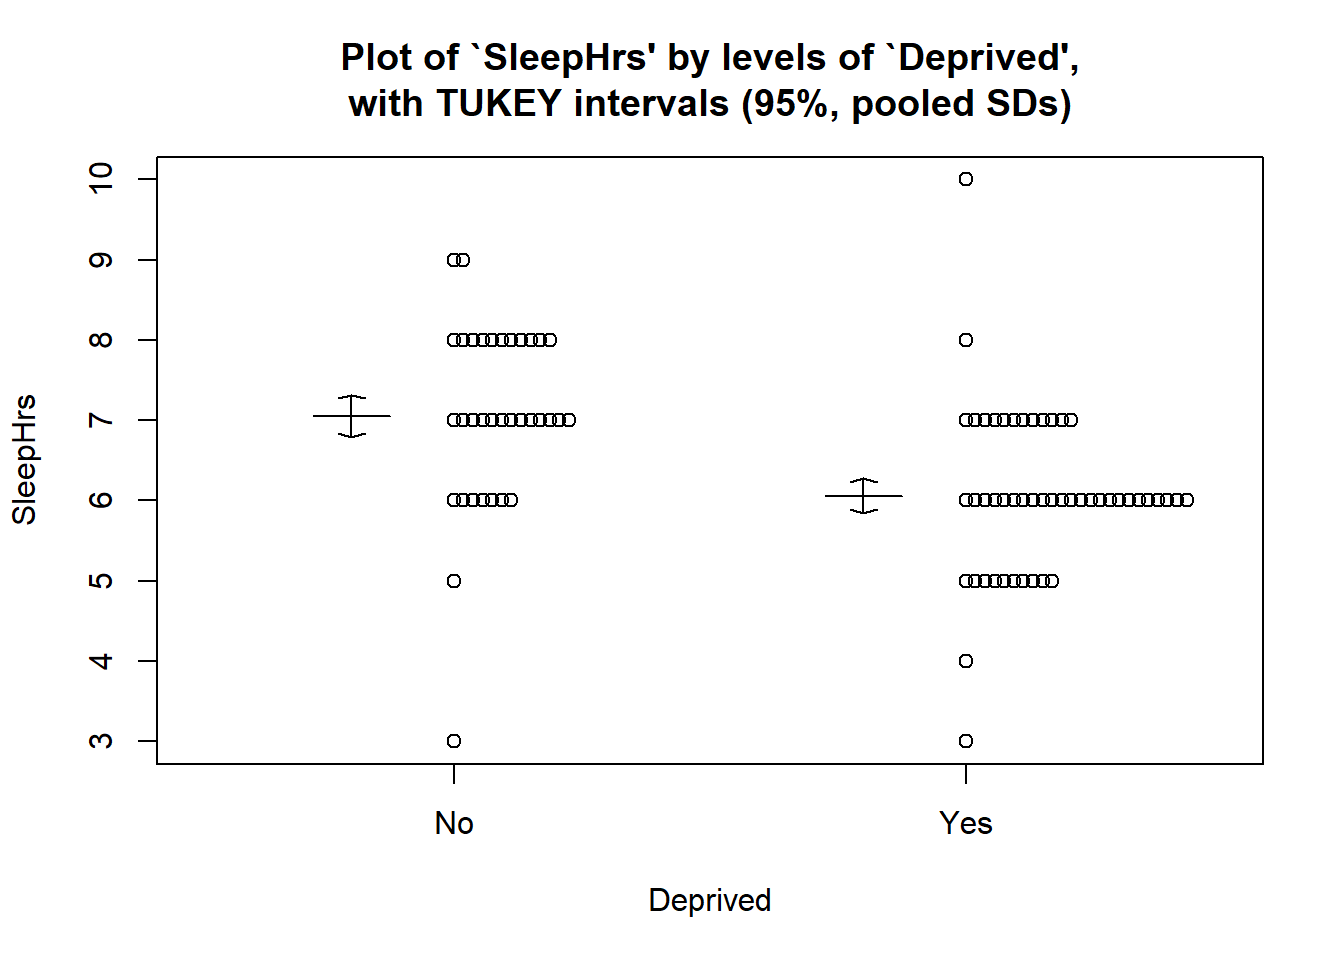
\includegraphics{Engsci211assignment2_task3_files/figure-latex/unnamed-chunk-7-1.pdf}

\begin{Shaded}
\begin{Highlighting}[]
\KeywordTok{summary1way}\NormalTok{(delays.fit2)}
\end{Highlighting}
\end{Shaded}

\begin{verbatim}
## ANOVA Table:
##                 Df  Sum Squares  Mean Square  F-statistic  p-value   
## Between Groups  3   36.84011     12.28004     6.41477      4e-04     
## Within Groups   156 298.63672    1.91434                             
## Total           159 335.47683                                        
## 
## Numeric Summary:
##           Sample size     Mean  Median  Std Dev  Midspread
## All Data          160  2.44298 2.44140  1.45256    2.03104
## Alaska             40  2.40619 2.07944  1.20484    1.88574
## American           40  2.98300 2.91741  1.53359    1.96359
## Delta              40  1.69067 1.38629  1.40075    2.15258
## United             40  2.69208 2.60200  1.37540    1.79764
## 
## Table of Effects: (GrandMean and deviations from GM)
##  typ.val   Alaska American    Delta   United 
##  2.44298 -0.03680  0.54001 -0.75232  0.24910
\end{verbatim}

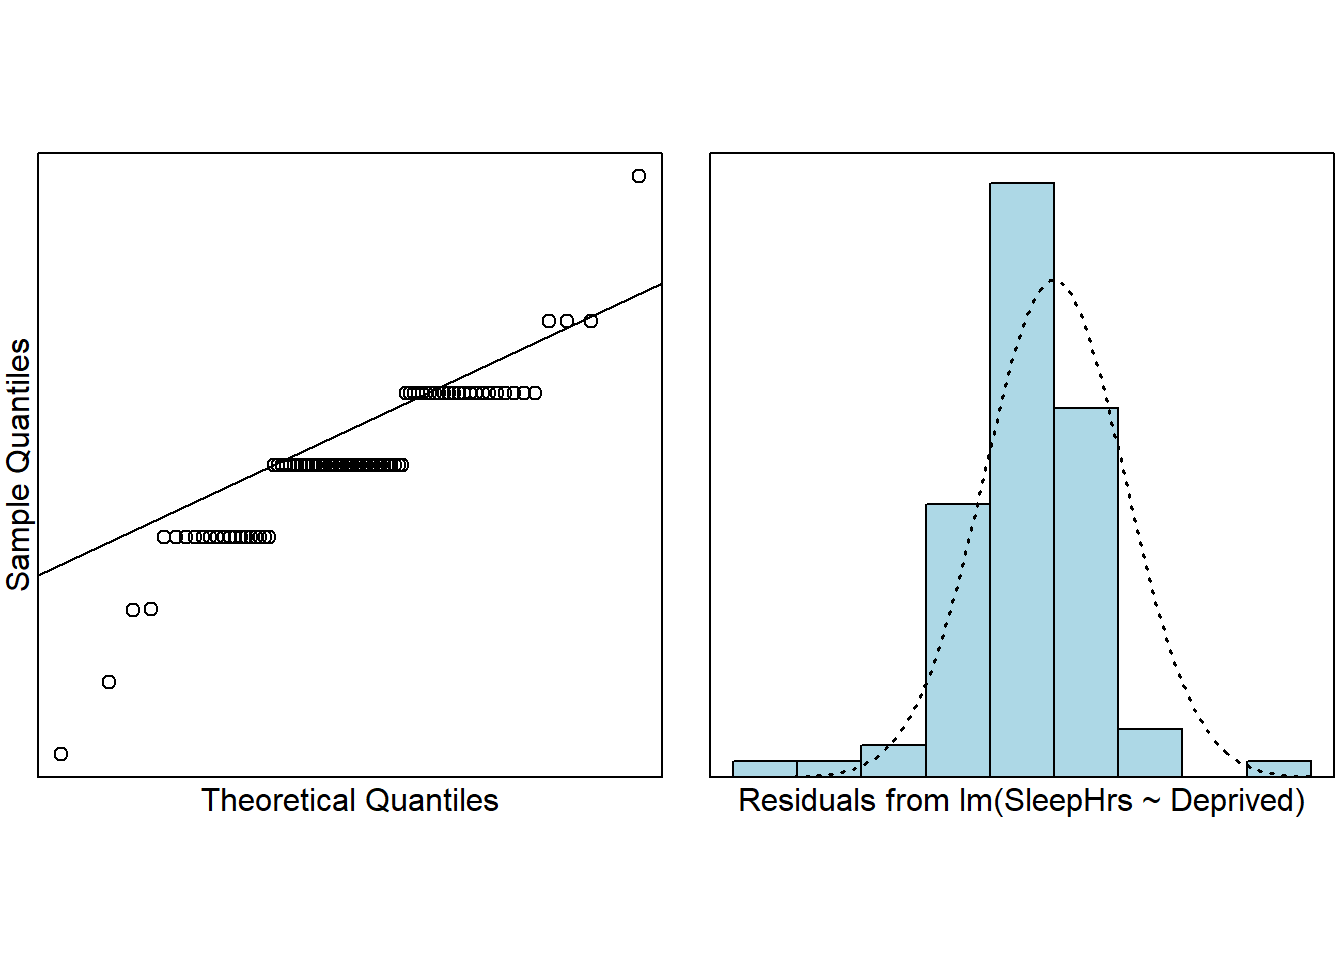
\includegraphics{Engsci211assignment2_task3_files/figure-latex/unnamed-chunk-8-1.pdf}

\begin{Shaded}
\begin{Highlighting}[]
\KeywordTok{cooks20x}\NormalTok{(delays.fit2)}
\end{Highlighting}
\end{Shaded}

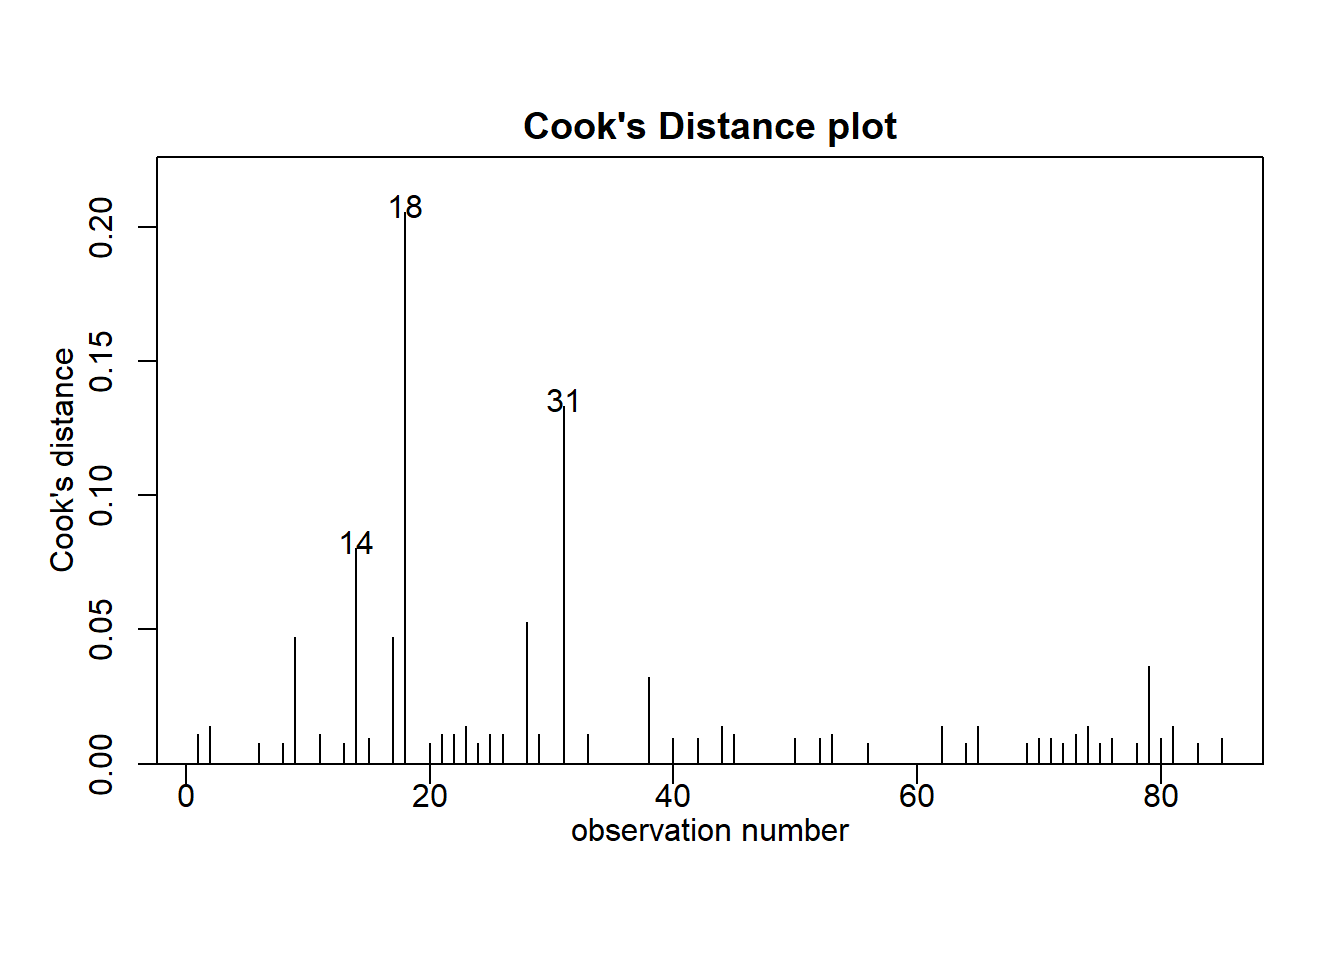
\includegraphics{Engsci211assignment2_task3_files/figure-latex/unnamed-chunk-8-2.pdf}

\begin{Shaded}
\begin{Highlighting}[]
\KeywordTok{multipleComp}\NormalTok{(delays.fit2)}
\end{Highlighting}
\end{Shaded}

\begin{verbatim}
##                       Estimate Tukey.L Tukey.U Tukey.p
## Alaska  -  American -0.5768106 -1.3803  0.2266  0.2477
## Alaska  -  Delta     0.7155220 -0.0879  1.5190  0.0995
## Alaska  -  United   -0.2858957 -1.0893  0.5175  0.7920
## American  -  Delta   1.2923326  0.4889  2.0958  0.0003
## American  -  United  0.2909149 -0.5125  1.0944  0.7832
## Delta  -  United    -1.0014177 -1.8049 -0.1980  0.0080
\end{verbatim}

\begin{Shaded}
\begin{Highlighting}[]
\KeywordTok{exp}\NormalTok{(}\KeywordTok{multipleComp}\NormalTok{(delays.fit2))[,}\DecValTok{1}\OperatorTok{:}\DecValTok{3}\NormalTok{]}
\end{Highlighting}
\end{Shaded}

\begin{verbatim}
##                      Estimate   Tukey.L   Tukey.U
## Alaska  -  American 0.5616869 0.2515031 1.2543280
## Alaska  -  Delta    2.0452540 0.9158525 4.5676553
## Alaska  -  United   0.7513410 0.3364519 1.6778278
## American  -  Delta  3.6412703 1.6305217 8.1319439
## American  -  United 1.3376507 0.5989962 2.9873897
## Delta  -  United    0.3673583 0.1644909 0.8203699
\end{verbatim}

\hypertarget{methods-and-assumption-checks}{%
\subsubsection{\texorpdfstring{\textbf{Methods and Assumption
Checks}}{Methods and Assumption Checks}}\label{methods-and-assumption-checks}}

We a numerical method made on four groups, so we should use a one-way
ANOVA / linear regression model.

Our model is:
\[\log({\tt dep-delays})_{i} = \beta_0 + \beta_1 \times {\tt america + \beta_2 \times {\tt delta} + \beta_3 \times {\tt united} + \varepsilon{i}\]


\end{document}
